%%
%% FuzzRSP: A Multi-Phase Fuzzing Framework for the SGP.22 RSP Protocol Stack
%% Submitted to ICT Express
%%

\documentclass[final,3p,times,twocolumn]{elsarticle}

\usepackage{blindtext, graphicx, amsmath, algorithm, algpseudocode,
            pifont, algcompatible, comment, layout, amsthm, amssymb}
\usepackage{enumitem}
\usepackage{eso-pic}
\usepackage{booktabs}
\usepackage{float}
\usepackage{tikz}
\usetikzlibrary{arrows.meta, shapes.geometric, positioning, fit, backgrounds, calc}
\usepackage{listings}
\usepackage{xcolor}

%% Listing colour palette (readable on light grey background)
\definecolor{lstkey}{HTML}{0B4F6C}
\definecolor{lstcmt}{HTML}{2E7D32}
\definecolor{lststr}{HTML}{C2410C}
\definecolor{lstprompt}{HTML}{1565C0}
\definecolor{lstresp}{HTML}{00695C}
\definecolor{lstwarn}{HTML}{C62828}

%% Base frame (shared by all listing styles)
\lstdefinestyle{termstyle}{
  basicstyle=\ttfamily\scriptsize,
  backgroundcolor=\color{gray!8},
  frame=single,
  framerule=0.4pt,
  rulecolor=\color{gray!50},
  breaklines=true,
  breakatwhitespace=false,
  keepspaces=true,
  columns=fullflexible,
  xleftmargin=4pt,
  xrightmargin=4pt,
  aboveskip=4pt,
  belowskip=2pt,
  showstringspaces=false,
  upquote=true
}

%% C source (Finding~1)
\lstdefinestyle{codestyle}{
  style=termstyle,
  language=C,
  keywordstyle=\color{lstkey}\bfseries,
  commentstyle=\color{lstcmt}\itshape,
  stringstyle=\color{lststr},
  identifierstyle=\color{black}
}

%% ASAN / sanitizer log output
\lstdefinestyle{asanstyle}{
  style=termstyle,
  language={},
  sensitive=false,
  morekeywords={ERROR,READ,AddressSanitizer,heap-buffer-overflow},
  keywordstyle=\color{lstwarn}\bfseries,
  identifierstyle=\color{violet!55!black},
  commentstyle=\color{lstcmt}\itshape,
  stringstyle=\color{lststr}
}

%% Python-like tool output (Hypothesis, tracebacks)
\lstdefinestyle{pyoutstyle}{
  style=termstyle,
  language=Python,
  keywordstyle=\color{lstkey}\bfseries,
  commentstyle=\color{lstcmt}\itshape,
  stringstyle=\color{lststr},
  emph={AssertionError,Falsifying,None,error,wire_bytes,decoded,Incorrect,
        padding,binascii,b64decode},
  emphstyle=\color{lstwarn},
  morekeywords={File,line,Error}
}

%% TLS wire-format snippet (prompt / response markers)
\lstdefinestyle{tlslogstyle}{
  style=termstyle,
  language={},
  literate=
    {>>}{{\textcolor{lstprompt}{\textbf{>}{>}}}}2
    {<<}{{\textcolor{lstresp}{\textbf{<}{<}}}}2
}

\lstset{style=termstyle}
\renewcommand{\qedsymbol}{$\blacksquare$}

\usepackage[utf8]{inputenc}
\usepackage[english]{babel}
\usepackage{hyperref}
\hypersetup{colorlinks=true, linkcolor=black, filecolor=black, urlcolor=cyan}

\usepackage{caption}
\captionsetup{justification=raggedright, singlelinecheck=false}
\captionsetup[table]{labelformat=simple, labelsep=newline}
\captionsetup[figure]{labelformat=simple, labelsep=period}

\newtheorem{theorem}{Theorem}
\newtheorem{lemma}{Lemma}
\newtheorem{definition}{Definition}

\journal{ICT Express}

\begin{document}

\begin{frontmatter}

\title{FuzzRSP: A Multi-Phase Fuzzing Framework for the SGP.22 RSP Protocol Stack}

\author{Author's Full Name 1\corref{cor1}}
\ead{author1@institution.edu}

\author{Author's Full Name 2}
\ead{author2@institution.edu}

\author{Author's Full Name 3}
\ead{author3@institution.edu}

\address{Department of Computer Science and Engineering, Institution, City, Country}

\cortext[cor1]{Corresponding author}

\begin{abstract}
Remote SIM Provisioning (RSP) per GSMA SGP.22 is the protocol that enables
over-the-air eUICC profile management in billions of connected devices.
Despite its security-critical role, the RSP software stack has received
minimal systematic fuzzing attention.
We present \textit{FuzzRSP}, a multi-phase framework that applies four
complementary fuzzing techniques across the full RSP stack:
(1) AFL++ coverage-guided fuzzing of the lpac C library,
(2) Atheris and Hypothesis property-based testing of the osmo-smdpp Python server,
(3) tlsfuzzer protocol fuzzing of a post-quantum TLS proxy (OpenSSL 3.6.0,
X25519MLKEM768), and
(4) advanced techniques comprising a differential C/Python ASN.1 oracle,
a state-machine-aware HTTP fuzzer, and grammar-guided DER mutation.
Across 3.17 billion AFL++ executions and 443 additional targeted probes, we
confirm four security findings: a heap buffer overread in the eUICC client,
a Python ASN.1 CHOICE decoder crash, a TLS alert code non-conformance in
OpenSSL's hybrid post-quantum path, and incomplete error handling in the
SM-DP+ server's HTTP interface.
\end{abstract}

\begin{keyword}
fuzzing \sep eUICC \sep remote SIM provisioning \sep post-quantum TLS \sep
protocol security \sep differential testing
\end{keyword}

\end{frontmatter}

%% ================================================================
\section{Introduction}\label{sec:intro}
%% ================================================================

Remote SIM Provisioning (RSP), standardised by GSMA as SGP.22~\cite{gsma_sgp22},
enables over-the-air management of embedded SIM (eUICC) profiles in smartphones,
IoT devices, and automotive systems.
The RSP protocol stack spans a client library running on the device (LPA), an
SM-DP+ provisioning server reachable over HTTPS, and a chain of cryptographically
verified ASN.1 messages encoding profile data, X.509 certificates, and BER-TLV
binary structures.
Any parsing vulnerability in this stack can be triggered remotely by a malicious
or compromised SM-DP+ server, making it a high-value attack surface.

Despite this risk, the RSP codebase has received little systematic
fuzzing~\cite{aflpp,klees2018evaluating}.
Prior work on IoT firmware fuzzing~\cite{firmfuzz,chen2016towards} and
protocol fuzzing~\cite{tlsfuzzer_repo,pham2020aflnet} rarely targets
proprietary GSMA-defined binary protocols.
The recent standardisation of post-quantum cryptography~\cite{nist_fips203,
nist_fips204} introduces additional urgency: production RSP servers are beginning
to deploy ML-KEM and ML-DSA, but no published fuzzing study covers these
algorithms at the TLS layer.

We present \textbf{FuzzRSP}, a multi-phase framework that
systematically covers the full RSP stack through four coordinated phases:
coverage-guided C fuzzing (AFL++~\cite{aflpp}), Python property-based testing
(Hypothesis~\cite{hypothesis}, Atheris~\cite{atheris}), PQ-TLS protocol fuzzing
(tlsfuzzer~\cite{tlsfuzzer_repo}), and three advanced harnesses: a
differential C/Python DER oracle, a state-machine-aware HTTP fuzzer, and a
grammar-guided mutation engine.

Our contributions are:
\begin{enumerate}[leftmargin=*,topsep=2pt,itemsep=0pt]
\item The first systematic fuzzing study of the SGP.22 RSP protocol stack covering
  all three trust boundaries (device, server, transport).
\item Four confirmed security findings including a heap buffer overread
  (CVE-class) in a widely-deployed eUICC client library and a Python ASN.1
  CHOICE decoder crash exploitable in under two bytes.
\item The first fuzzing evaluation of X25519MLKEM768 hybrid key exchange in
  production OpenSSL 3.6.0, testing 384 individual ML-KEM coefficient positions.
\item A reusable differential oracle design exposing parser disagreements between
  a C TLV walker and a Python schema-based decoder on the same wire messages.
\end{enumerate}

%% ================================================================
\section{Background}\label{sec:background}
%% ================================================================

\subsection{SGP.22 RSP Protocol}

The RSP protocol defines five ES9+ HTTP endpoints through which the LPA (on-device)
and SM-DP+ (server) negotiate profile download~\cite{gsma_sgp22}:
\texttt{initiateAuthentication} $\rightarrow$
\texttt{authenticateClient} $\rightarrow$
\texttt{getBoundProfilePackage} $\rightarrow$
\texttt{handleNotification} / \texttt{cancelSession}.
Each call carries base64-encoded ASN.1 DER blobs validated with ECDSA or (in newer
deployments) ML-DSA.
The binary profile itself is delivered as a Bound Profile Package (BPP), a BER-TLV
structure ~4 kB in size.

\subsection{Target Software}

\textbf{lpac}~\cite{lpac} is an open-source LPA written in C that parses all
server-supplied DER messages using a custom TLV walker (\texttt{euicc\_derutil\_*}).
\textbf{osmo-smdpp}~\cite{osmocom} is the Osmocom SM-DP+ server implemented
in Python/Twisted, decoding messages via the \texttt{asn1tools}
library~\cite{asn1tools}.
The PQ-TLS proxy is nginx 1.26.3 built against OpenSSL 3.6.0 with native support
for ML-KEM-768 and ML-DSA-44~\cite{openssl_pqc}.

\subsection{Fuzzing Background and Related Work}

Coverage-guided fuzzing~\cite{aflpp,libfuzzer} instruments code to track
which branches are exercised, guiding mutation toward new paths.
Property-based testing~\cite{hypothesis} generates structured inputs
satisfying user-defined invariants.
Differential fuzzing~\cite{differential_testing} feeds the same input to multiple
implementations and flags divergent outputs as potential bugs.
Grammar-guided fuzzing~\cite{grammarfuzz} restricts mutations to syntactically
valid structures, reaching deeper program paths.

\textbf{Related work.}
Stateful protocol fuzzing has advanced significantly through network-oriented
extensions of coverage-guided tools.
AFLNet~\cite{pham2020aflnet} augments AFL++ with response-feedback state
inference to guide fuzzing of TCP/IP servers.
StateAFL~\cite{natella2022stateafl} instruments in-process memory snapshots to
recover protocol state automatically without protocol-specific modelling.
IoTFuzzer~\cite{firmfuzz} and FIRMADYNE~\cite{chen2016towards} target embedded
firmware images through companion app analysis or full-system emulation.
None of these works address the GSMA SGP.22 binary protocol standard, the
eUICC client library attack surface, or post-quantum TLS at the wire level.
FuzzRSP bridges these gaps by combining static, dynamic, and differential
techniques across three distinct trust boundaries of a production RSP stack.

%% ================================================================
\section{FuzzRSP Architecture}\label{sec:design}
%% ================================================================

Fig.~\ref{fig:arch} illustrates the FuzzRSP four-phase architecture.
Each phase targets a distinct trust boundary of the RSP stack.

\begin{figure*}[t]
\centering
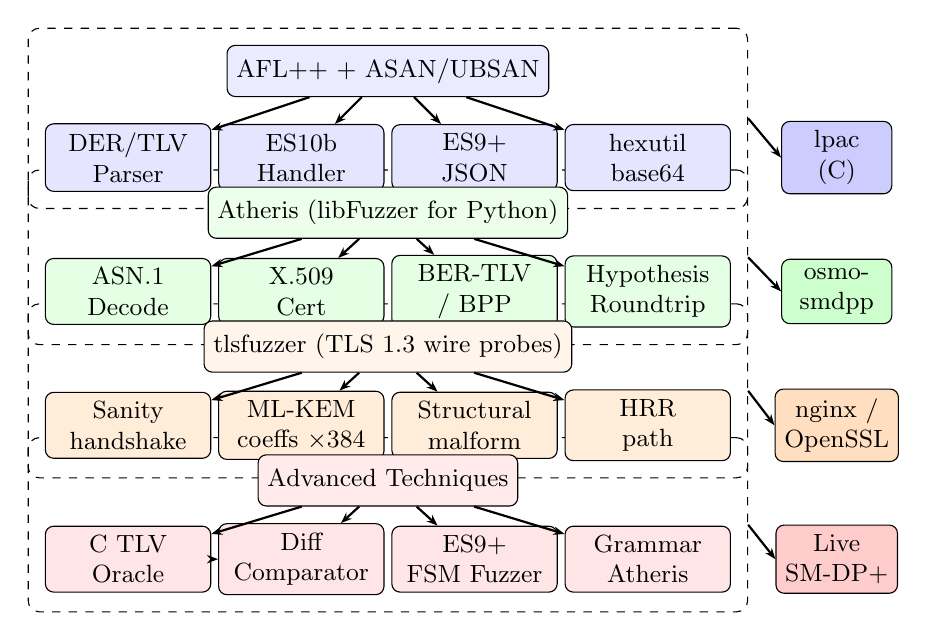
\begin{tikzpicture}[
  font=\small,
  box/.style={draw, rounded corners=3pt, minimum width=2.1cm,
              minimum height=0.65cm, align=center, fill=white},
  phase/.style={draw, rounded corners=4pt, dashed, inner sep=6pt},
  arrow/.style={-{Stealth[length=4pt]}, thick},
  label/.style={font=\footnotesize\itshape}
]

%% Phase 1: C AFL++
\node[box, fill=blue!10] (der)     at (0,3.5)   {DER/TLV\\Parser};
\node[box, fill=blue!10] (es10b)   at (2.2,3.5) {ES10b\\Handler};
\node[box, fill=blue!10] (es9p)    at (4.4,3.5) {ES9+\\JSON};
\node[box, fill=blue!10] (hexutil) at (6.6,3.5) {hexutil\\base64};
\node[box, fill=blue!8]  (afl)     at (3.3,4.6) {AFL++ + ASAN/UBSAN};
\draw[arrow] (afl) -- (der);
\draw[arrow] (afl) -- (es10b);
\draw[arrow] (afl) -- (es9p);
\draw[arrow] (afl) -- (hexutil);

\begin{pgfonlayer}{background}
\node[phase, fit=(der)(es10b)(es9p)(hexutil)(afl),
      label=above:{\textbf{Phase 1: lpac/euicc (C)}}] (p1) {};
\end{pgfonlayer}

%% Phase 2: Python
\node[box, fill=green!10] (asn1d)  at (0,1.8)   {ASN.1\\Decode};
\node[box, fill=green!10] (x509)   at (2.2,1.8) {X.509\\Cert};
\node[box, fill=green!10] (bertlv) at (4.4,1.8) {BER-TLV\\/ BPP};
\node[box, fill=green!10] (hyp)    at (6.6,1.8) {Hypothesis\\Roundtrip};
\node[box, fill=green!8]  (atheris) at (3.3,2.8) {Atheris (libFuzzer for Python)};
\draw[arrow] (atheris) -- (asn1d);
\draw[arrow] (atheris) -- (x509);
\draw[arrow] (atheris) -- (bertlv);
\draw[arrow] (atheris) -- (hyp);

\begin{pgfonlayer}{background}
\node[phase, fit=(asn1d)(x509)(bertlv)(hyp)(atheris),
      label=above:{\textbf{Phase 2: osmo-smdpp (Python)}}] (p2) {};
\end{pgfonlayer}

%% Phase 3: PQ-TLS
\node[box, fill=orange!15] (sanity) at (0,0.1)   {Sanity\\handshake};
\node[box, fill=orange!15] (mlkem)  at (2.2,0.1) {ML-KEM\\coeffs $\times$384};
\node[box, fill=orange!15] (struct) at (4.4,0.1) {Structural\\malform};
\node[box, fill=orange!15] (hrr)    at (6.6,0.1) {HRR\\path};
\node[box, fill=orange!8]  (tls)    at (3.3,1.1) {tlsfuzzer (TLS 1.3 wire probes)};
\draw[arrow] (tls) -- (sanity);
\draw[arrow] (tls) -- (mlkem);
\draw[arrow] (tls) -- (struct);
\draw[arrow] (tls) -- (hrr);

\begin{pgfonlayer}{background}
\node[phase, fit=(sanity)(mlkem)(struct)(hrr)(tls),
      label=above:{\textbf{Phase 3: PQ-TLS / nginx}}] (p3) {};
\end{pgfonlayer}

%% Phase 4: Advanced
\node[box, fill=red!10]  (oracle)  at (0,-1.6)   {C TLV\\Oracle};
\node[box, fill=red!10]  (diff)    at (2.2,-1.6) {Diff\\Comparator};
\node[box, fill=red!10]  (fsm)     at (4.4,-1.6) {ES9+\\FSM Fuzzer};
\node[box, fill=red!10]  (grammar) at (6.6,-1.6) {Grammar\\Atheris};
\node[box, fill=red!8]   (adv)     at (3.3,-0.6) {Advanced Techniques};
\draw[arrow] (adv) -- (oracle);
\draw[arrow] (adv) -- (diff);
\draw[arrow] (adv) -- (fsm);
\draw[arrow] (adv) -- (grammar);
\draw[arrow, dashed] (oracle) -- (diff);

\begin{pgfonlayer}{background}
\node[phase, fit=(oracle)(diff)(fsm)(grammar)(adv),
      label=above:{\textbf{Phase 4: Differential / FSM / Grammar}}] (p4) {};
\end{pgfonlayer}

%% Target stack on right
\node[box, fill=blue!20,  minimum width=1.4cm] (lpac_t)  at (9.0, 3.5) {lpac\\(C)};
\node[box, fill=green!20, minimum width=1.4cm] (smdpp_t) at (9.0, 1.8) {osmo-\\smdpp};
\node[box, fill=orange!25,minimum width=1.4cm] (tls_t)   at (9.0, 0.1) {nginx /\\OpenSSL};
\node[box, fill=red!20,   minimum width=1.4cm] (adv_t)   at (9.0,-1.6) {Live\\SM-DP+};

\draw[arrow] (p1.east) -- (lpac_t.west);
\draw[arrow] (p2.east) -- (smdpp_t.west);
\draw[arrow] (p3.east) -- (tls_t.west);
\draw[arrow] (p4.east) -- (adv_t.west);

\end{tikzpicture}
\caption{FuzzRSP architecture. Four phases target distinct RSP trust boundaries.
Arrows indicate fuzz inputs reaching their target component.}
\label{fig:arch}
\end{figure*}

\subsection{Phase 1: Coverage-Guided C Fuzzing}

Six AFL++ harnesses instrument the lpac euicc library with AddressSanitizer
and UndefinedBehaviorSanitizer.
A separate CMPLOG build is used for comparison-operand logging~\cite{aflpp}.
Edge coverage is measured via AFL++'s shared-memory bitmap instrumentation;
percentages in Table~\ref{tab:afl} reflect the fraction of all discovered
branch-pair edges relative to the harness-specific total reported by
\texttt{afl-cmin}.
The harnesses cover raw DER parsing (\texttt{fuzz\_derutil}), server-parameter
message chains (\texttt{fuzz\_es10b\_response}), ES9+ JSON parsing
(\texttt{fuzz\_es9p\_json}), profile metadata (\texttt{fuzz\_es8p\_metadata}),
profile list decoding (\texttt{fuzz\_es10c\_profiles}), and hexadecimal/base64
utilities (\texttt{fuzz\_hexutil}).

\subsection{Phase 2: Python Fuzzing and Property Testing}

Three Atheris harnesses target the SM-DP+ Python server: ASN.1 decoding of
six SGP.22 message types via \texttt{asn1tools}~\cite{asn1tools}, X.509
certificate chain and extension parsing, and BER-TLV / BoundProfilePackage
decoding.
A Hypothesis suite of ten property-based tests checks encode/decode
round-trip symmetry across eight SGP.22 types.

\subsection{Phase 3: PQ-TLS Protocol Fuzzing}

A custom tlsfuzzer harness sends 400 crafted TLS 1.3 ClientHello messages
to nginx/OpenSSL 3.6.0 configured with an ML-DSA-44 certificate and
X25519MLKEM768 key exchange.
Probe groups cover full handshakes, structural key-share malformations,
all 384 NTT coefficient positions of the ML-KEM-768 public key
(\texttt{t\_hat} array), classical X25519 edge cases, hybrid-structure
attacks, and the Hello Retry Request (HRR) path.

\subsection{Phase 4: Advanced Techniques}

\textbf{Differential oracle.}
\texttt{oracle\_lpac.c} reads raw DER bytes and applies the same C
\texttt{euicc\_derutil\_*} walk used by lpac, emitting structured JSON.
\texttt{diff\_lpac\_pysim.py} runs this binary as a subprocess, simultaneously
decodes the same bytes with \texttt{rsp.asn1.decode()}, and classifies each
result as \textit{agree-accept}, \textit{agree-reject}, \textit{split-C-accept},
\textit{split-PY-accept}, or \textit{semantic-split}~\cite{differential_testing}.
Algorithm~\ref{alg:oracle} formalises this classification.

\begin{algorithm}[t]
\caption{Differential ASN.1 Oracle (input: bytes $b$, type $T$)}\label{alg:oracle}
\begin{algorithmic}[1]
\State $r_C   \gets \texttt{oracle\_lpac}(b)$
\State $r_{Py}\gets \texttt{rsp.asn1.decode}(T, b)$
\If{both raise}
    \State \textbf{return} \textit{agree-reject}
\ElsIf{neither raises}
    \If{$\text{normalise}(r_C) = \text{normalise}(r_{Py})$}
        \State \textbf{return} \textit{agree-accept}
    \Else
        \State \textbf{return} \textit{semantic-split} \textbf{[flag]}
    \EndIf
\ElsIf{only $r_C$ succeeds}
    \State \textbf{return} \textit{split-C-accept}
\Else
    \State \textbf{return} \textit{split-PY-accept} \textbf{[flag]}
\EndIf
\end{algorithmic}
\end{algorithm}

\textbf{FSM-aware HTTP fuzzer.}
The ES9+ protocol has a strict five-state ordering
(Fig.~\ref{fig:fsm}).
\texttt{fuzz\_smdpp\_fsm.py} models this FSM and exercises six strategies:
happy-path baseline, skip-state attacks, replay after \texttt{cancelSession},
per-state ASN.1 payload mutation, concurrent session cross-use, and
boundary values for \texttt{transactionId} (null, empty, 4096-char, Unicode,
path traversal, SQL-shaped strings).

\textbf{Grammar-guided Atheris.}
\texttt{fuzz\_asn1\_grammar.py} implements a libFuzzer custom mutator that
operates in DER-space rather than byte-space: decode a seed into a Python dict,
apply one of five structural mutations (flip optional field, boundary integer,
truncate octet string, swap CHOICE branch, inject duplicate key), re-encode
to DER, then feed the result as the fuzz target.

\begin{figure}[t]
\centering
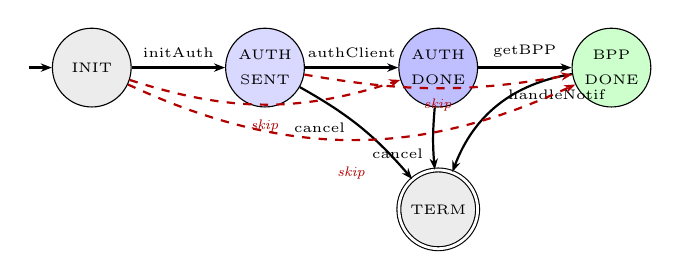
\begin{tikzpicture}[
  font=\small,
  state/.style={draw, circle, minimum size=1.0cm, align=center,
                inner sep=1pt, fill=white},
  illegal/.style={-{Stealth[length=4pt]}, dashed, red!70!black, thick},
  normal/.style={-{Stealth[length=4pt]}, thick},
  selfarrow/.style={loop above, -{Stealth[length=4pt]}, thick}
]

\node[state, fill=gray!15]     (init)  at (0,0)    {\tiny INIT};
\node[state, fill=blue!15]     (auth1) at (2.2,0)  {\tiny AUTH\\[-2pt]\tiny SENT};
\node[state, fill=blue!25]     (auth2) at (4.4,0)  {\tiny AUTH\\[-2pt]\tiny DONE};
\node[state, fill=green!20]    (bpp)   at (6.6,0)  {\tiny BPP\\[-2pt]\tiny DONE};
\node[state, fill=gray!15,
      double, double distance=1pt] (term) at (4.4,-1.8)  {\tiny TERM};

\draw[normal] (-0.8,0) -- (init);
\draw[normal] (init)  -- node[above]{\tiny initAuth}  (auth1);
\draw[normal] (auth1) -- node[above]{\tiny authClient} (auth2);
\draw[normal] (auth2) -- node[above]{\tiny getBPP}     (bpp);
\draw[normal] (bpp)   to[bend right=30]
              node[right,yshift=4pt]{\tiny handleNotif} (term);
\draw[normal] (auth1) to[bend left=10]
              node[left, xshift=-2pt]{\tiny cancel} (term);
\draw[normal] (auth2) to[bend right=5]
              node[below left]{\tiny cancel} (term);

%% Illegal skip-state edges
\draw[illegal] (init)  to[bend right=18]
               node[below, yshift=-2pt]{\tiny \textit{skip}}  (auth2);
\draw[illegal] (init)  to[bend right=25]
               node[below, yshift=-6pt]{\tiny \textit{skip}}  (bpp);
\draw[illegal] (auth1) to[bend right=10]
               node[below]{\tiny \textit{skip}} (bpp);

\end{tikzpicture}
\caption{ES9+ RSP protocol finite-state machine modelled in FuzzRSP Phase~4.
Solid arrows show valid transitions; dashed red arrows show skip-state
attacks probed by \texttt{fuzz\_smdpp\_fsm.py}.}
\label{fig:fsm}
\end{figure}

%% ================================================================
\section{Results}\label{sec:results}
%% ================================================================

\subsection{Phase 1: AFL++ Campaign on lpac}

Table~\ref{tab:afl} summarises the AFL++ campaign across 16.6 to 18.2 hours of
runtime per long-running harness, totalling approximately \textbf{3.17 billion}
executions.

\begin{table}[h]
\centering
\caption{AFL++ campaign summary. Hangs indicate confirmed freeze inputs; all
arise from Finding~1. Execs in millions (M) or billions (B).}
\label{tab:afl}
\begin{tabular}{@{}lrrr@{}}
\toprule
Harness & Execs & Edge Cov. & Hangs \\
\midrule
\texttt{fuzz\_derutil}      & 47M    & 15.6\% & 0  \\
\texttt{fuzz\_es10b} (×2)   & 703M   & 19.4\% & 0  \\
\texttt{fuzz\_es9p\_json}   & 1.39B  & 7.1\%  & 0  \\
\texttt{fuzz\_es8p\_meta}   & 19M    & 28.7\% & \textbf{28} \\
\texttt{fuzz\_es10c\_prof}  & 954M   & 17.3\% & \textbf{29} \\
\texttt{fuzz\_hexutil}      & 67M    & 47.6\% & 0  \\
\bottomrule
\end{tabular}
\end{table}

\textbf{Finding 1 (High): Heap buffer overread in \texttt{euicc\_hexutil\_bin2gsmbcd}.}
A zero-length ICCID TLV (\texttt{5A 00}) causes \texttt{euicc\_hexutil\_bin2hex}
to return \texttt{n=0}; the subsequent \texttt{n-=1} underflows to \texttt{-1}
which, cast to \texttt{uint32\_t}, becomes \texttt{4,294,967,295}, and the loop
bound passed to \texttt{gsmbcd\_swap\_chars}, reading billions of bytes past
the heap allocation.
This is a remotely triggerable heap buffer overread (CWE-125).
At minimum it enables a Denial of Service (DoS) of the LPA process from any
rogue or compromised SM-DP+ operator; heap-layout-dependent exploitation may
further expose adjacent allocation contents to the attacker (CVE-class: High).
The vulnerable code path in \texttt{hexutil.c} is shown in
Listing~\ref{lst:vuln_c}, and the ASAN crash report in
Listing~\ref{lst:asan}.

\begin{lstlisting}[style=codestyle,caption={Vulnerable code in \texttt{euicc\_hexutil\_bin2gsmbcd} (hexutil.c lines 101 to 114). Line 3 underflows when \texttt{bin\_len=0}.},label=lst:vuln_c]
int n = euicc_hexutil_bin2hex(
    output, output_len, bin, bin_len);
if (n < 0) { return -1; }
n -= 1;   // BUG: n=0 -> n=-1 (signed)
gsmbcd_swap_chars(output,
    (uint32_t)n); // cast: 4294967295
\end{lstlisting}

\begin{lstlisting}[style=asanstyle,caption={ASAN heap-buffer-overflow report. The read originates in \texttt{gsmbcd\_swap\_chars} called from the profile metadata parser.},label=lst:asan]
ERROR: AddressSanitizer:
  heap-buffer-overflow on address
  0x50c0000000c0
READ of size 1 at 0x50c0000000c0
    #0 gsmbcd_swap_chars  hexutil.c:20
    #1 euicc_hexutil_bin2gsmbcd
                          hexutil.c:108
    #2 es8p_metadata_parse es8p.c:184
\end{lstlisting}

\begin{figure}[h]
\centering
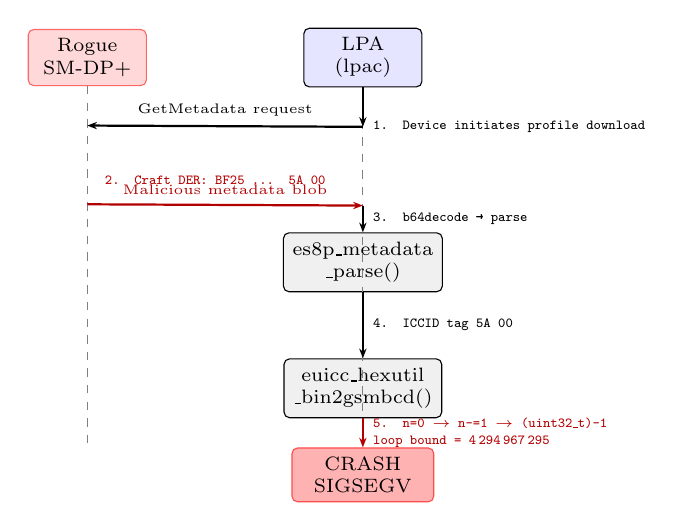
\begin{tikzpicture}[
  font=\scriptsize,
  actor/.style={draw, rectangle, rounded corners=2pt,
                minimum width=1.5cm, minimum height=0.45cm,
                align=center, fill=white},
  rogue/.style={actor, fill=red!15, draw=red!60},
  device/.style={actor, fill=blue!10},
  func/.style={actor, fill=gray!12, minimum width=2.0cm},
  msg/.style={-{Stealth[length=3.5pt]}, thick},
  badmsg/.style={-{Stealth[length=3.5pt]}, thick, red!70!black},
  crash/.style={actor, fill=red!30, draw=red!70, minimum width=1.8cm},
  note/.style={font=\tiny\ttfamily, align=left}
]

%% Actors (column x positions)
\node[rogue]  (smdp)   at (0, 0)    {Rogue\\SM-DP+};
\node[device] (lpa)    at (3.5, 0)  {LPA\\(lpac)};
\node[func]   (parser) at (3.5,-2.6){es8p\_metadata\\\_parse()};
\node[func]   (hexutil)at (3.5,-4.2){euicc\_hexutil\\\_bin2gsmbcd()};

%% Lifelines
\draw[dashed, gray] (smdp)    -- ++(0,-5.0);
\draw[dashed, gray] (lpa)     -- ++(0,-5.0);

%% Step 1: device initiates download
\draw[msg] (lpa.south)+(0,0) -- ++(0,-0.5)
    node[right, note]{1. Device initiates profile download};
\draw[msg] ($(lpa.south)+(0,-0.5)$) -- ($(smdp.south)+(0,-0.5)$)
    node[midway, above, font=\tiny]{GetMetadata request};

%% Step 2: rogue crafts response
\node[note, red!70!black] at ($(smdp.south)+(0,-1.2)$) [right=0.1cm]
    {2. Craft DER: \texttt{BF25 ... 5A 00}};
\draw[badmsg] ($(smdp.south)+(0,-1.5)$) -- ($(lpa.south)+(0,-1.5)$)
    node[midway, above, font=\tiny, red!70!black]
    {Malicious metadata blob};

%% Step 3: LPA parses
\draw[msg] ($(lpa.south)+(0,-1.5)$) -- (parser.north)
    node[midway, right, note]{3. b64decode → parse};

%% Step 4: zero-len ICCID reaches hexutil
\draw[msg] (parser.south) -- (hexutil.north)
    node[midway, right, note]{4. ICCID tag \texttt{5A 00}};

%% Step 5: crash
\node[crash] (boom) at (3.5,-5.3) {CRASH\\SIGSEGV};
\draw[badmsg] (hexutil.south) -- (boom.north)
    node[midway, right, note, red!70!black]
    {5. \texttt{n=0} $\to$ \texttt{n-=1} $\to$ \texttt{(uint32\_t)-1}\\
        loop bound = 4\,294\,967\,295};

\end{tikzpicture}
\caption{Attack flow for Finding~1. A rogue SM-DP+ embeds a zero-length ICCID
TLV (\texttt{5A~00}) in a crafted metadata response.
The LPA parses it without length validation, triggering a signed-integer
underflow and heap buffer overread.
\textbf{Fix:} guard \texttt{if (n == 0) return 0;} before \texttt{n -= 1}.}
\label{fig:attack1}
\end{figure}

\subsection{Phase 2: Python Fuzzing and Hypothesis}

\textbf{Finding 2 (Medium): \texttt{PendingNotification} CHOICE accepts \texttt{\textbackslash{}x00\textbackslash{}x00}.}
Hypothesis discovered that \texttt{rsp.asn1.decode('PendingNotification',}
\texttt{b'\textbackslash{}x00\textbackslash{}x00')} returns \texttt{(None,~None)} instead of
raising \texttt{DecodeError}.
The server subsequently calls \texttt{rsp.asn1.encode} on the degenerate
tuple, raising \texttt{EncodeError}, an unhandled exception at the
\texttt{handleNotification} endpoint.
The endpoint requires no prior authentication in osmo-smdpp's default
configuration, making this an unauthenticated remote crash (CWE-248,
CVE-class: Medium) exploitable with a two-byte HTTP payload.
Listing~\ref{lst:hypothesis} shows the Hypothesis falsifying example.

\begin{lstlisting}[style=pyoutstyle,caption={Hypothesis falsifying example for Finding~2. The two-byte input \texttt{0x00 0x00} is sufficient to crash the SM-DP+ \texttt{handleNotification} handler.},label=lst:hypothesis]
AssertionError: [Class A - Re-encode
 failure] asn1tools decoded
 PendingNotification but FAILED to
 re-encode the decoded value.
  wire_bytes = 0000
  decoded    = (None, None)
  error      = PendingNotification:
   Expected tuple(str,object),
   got (None, None).
Falsifying example:
  test_pending_notification_binary
  _roundtrip(data=b'\x00\x00')
\end{lstlisting}

\begin{figure}[h]
\centering
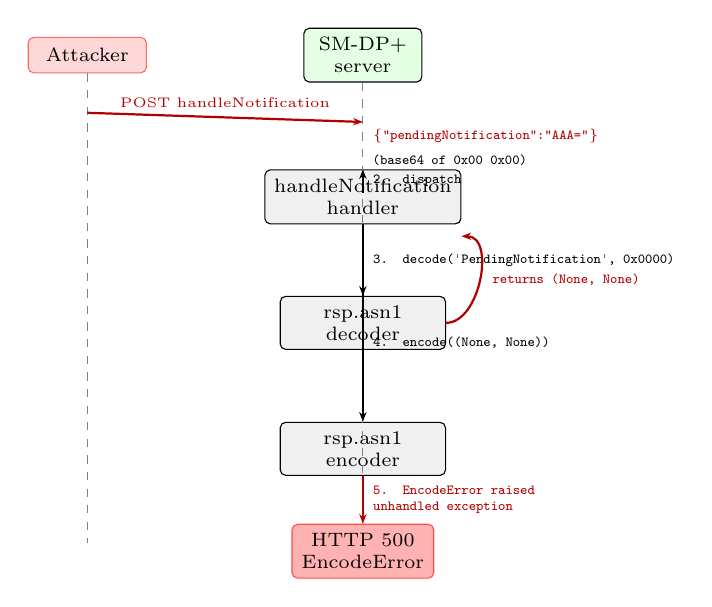
\begin{tikzpicture}[
  font=\scriptsize,
  actor/.style={draw, rectangle, rounded corners=2pt,
                minimum width=1.5cm, minimum height=0.45cm,
                align=center, fill=white},
  attacker/.style={actor, fill=red!15, draw=red!60},
  server/.style={actor, fill=green!10},
  layer/.style={actor, fill=gray!12, minimum width=2.1cm},
  msg/.style={-{Stealth[length=3.5pt]}, thick},
  badmsg/.style={-{Stealth[length=3.5pt]}, thick, red!70!black},
  crash/.style={actor, fill=red!30, draw=red!70, minimum width=1.8cm},
  note/.style={font=\tiny\ttfamily, align=left}
]

%% Actors
\node[attacker] (atk)    at (0, 0)    {Attacker};
\node[server]   (smdpp)  at (3.5, 0)  {SM-DP+\\server};
\node[layer]    (handler)at (3.5,-1.8){handleNotification\\handler};
\node[layer]    (asn1)   at (3.5,-3.4){rsp.asn1\\decoder};
\node[layer]    (enc)    at (3.5,-5.0){rsp.asn1\\encoder};

%% Lifelines
\draw[dashed, gray] (atk)   -- ++(0,-6.2);
\draw[dashed, gray] (smdpp) -- ++(0,-6.2);

%% Step 1: HTTP POST (no prior session required)
\draw[badmsg] ($(atk.south)+(0,-0.5)$) --
              ($(smdpp.south)+(0,-0.5)$)
    node[midway, above, font=\tiny, red!70!black]
    {POST handleNotification};
\node[note, red!70!black] at ($(atk.south)+(-0.1,-0.8)$) [right=3.6cm]
    {\{"pendingNotification":"AAA="\}};
\node[note] at ($(atk.south)+(-0.1,-1.1)$) [right=3.6cm]
    {(base64 of \texttt{0x00 0x00})};

%% Step 2: handler calls decode
\draw[msg] ($(smdpp.south)+(0,-1.4)$) -- (handler.north)
    node[midway, right, note]{2. dispatch};
\draw[msg] (handler.south) -- (asn1.north)
    node[midway, right, note]{3. decode(\textquotesingle PendingNotification\textquotesingle, \texttt{0x0000})};

%% Step 3: decoder returns (None,None)
\draw[badmsg] (asn1.east)+(0,0) to[out=0,in=0]
    node[right, note, red!70!black, xshift=1pt]{returns \texttt{(None, None)}}
    ($(handler.east)+(0,-0.5)$);

%% Step 4: handler calls encode
\draw[msg] ($(handler.south)+(0,-0.5)$) -- (enc.north)
    node[midway, right, note]{4. encode(\texttt{(None, None)})};

%% Step 5: EncodeError → 500
\node[crash] (err) at (3.5,-6.3) {HTTP 500\\EncodeError};
\draw[badmsg] (enc.south) -- (err.north)
    node[midway, right, note, red!70!black]
    {5. \texttt{EncodeError} raised\\unhandled exception};

\end{tikzpicture}
\caption{Attack flow for Finding~2. An unauthenticated HTTP POST with a 2-byte
\texttt{pendingNotification} payload (\texttt{0x00~0x00}) reaches the ASN.1
decoder, which returns a degenerate \texttt{(None,~None)} CHOICE value.
The subsequent re-encode raises \texttt{EncodeError}, crashing the request.
\textbf{Fix:} guard \texttt{if decoded[0] is None: raise ValueError}.}
\label{fig:attack2}
\end{figure}

Nine of ten round-trip tests passed; no DER malleability enabling
signature bypass was found.

\subsection{Phase 3: PQ-TLS Campaign}

Table~\ref{tab:tls} summarises the 400-probe tlsfuzzer campaign.

\begin{table}[h]
\centering
\caption{PQ-TLS tlsfuzzer probe results (400 total).}
\label{tab:tls}
\begin{tabular}{@{}lrrr@{}}
\toprule
Probe group & Count & Pass & Fail \\
\midrule
Sanity handshake      & 2   & 2   & 0 \\
Structural malform    & 5   & 4   & \textbf{1} \\
ML-KEM coefficient    & 384 & 384 & 0 \\
X25519 classical part & 4   & 4   & 0 \\
Hybrid structure      & 4   & 4   & 0 \\
HRR path              & 1   & 1   & 0 \\
\midrule
\textbf{Total}        & \textbf{400} & \textbf{399} & \textbf{1} \\
\bottomrule
\end{tabular}
\end{table}

\textbf{Finding 3 (Low): Wrong TLS alert for empty hybrid \texttt{key\_share}.}
A ClientHello with a zero-length \texttt{key\_exchange} for the
X25519MLKEM768 group elicits \texttt{decode\_error(50)} from OpenSSL 3.6.0
rather than the \texttt{illegal\_parameter(47)} required by RFC~8446~\cite{rfc8446}.
Listing~\ref{lst:tls_wire} shows the expected vs.\ actual alert.
The session closes correctly; the wrong code affects client-side diagnostic
branches and strict conformance test suites.
All 384 ML-KEM coefficient probes (one per NTT coefficient position in the
1152-byte \texttt{t\_hat} array, each set to the smallest invalid value
$q = 3329$) were correctly rejected with \texttt{illegal\_parameter},
confirming that OpenSSL's FIPS~203 range-check~\cite{nist_fips203} executes
before any memory-sensitive decapsulation.

\begin{lstlisting}[style=tlslogstyle,caption={TLS 1.3 wire exchange for Finding~3. OpenSSL 3.6.0 emits alert 50 (\texttt{decode\_error}) where RFC~8446 §6.2 specifies alert 47 (\texttt{illegal\_parameter}).},label=lst:tls_wire]
>> ClientHello
   key_share: X25519MLKEM768 (0x11ec)
   key_exchange: (0 bytes)  <- trigger

<< Expected: Alert(fatal,
     illegal_parameter, 47)
<< Actual:   Alert(fatal,
     decode_error, 50)
\end{lstlisting}

\subsection{Phase 4: Differential, FSM, and Grammar}

The differential oracle ran 18 comparisons (3 types $\times$ 6 corpus files).
One \textit{split-PY-accept} was detected: \texttt{s01\_server\_signed1.bin}
interpreted as \texttt{PendingNotification} was accepted by Python's
\texttt{asn1tools} despite having no valid notification envelope tag,
returning the \texttt{(None,None)} class of output already identified in
Finding~2.
This cross-validates the differential design: it independently re-discovers
the same bug class from a different harness direction.

\textbf{Finding 4 (Low): ES9+ error handling leaks server internals.}
The FSM fuzzer exercised all six strategies (Table~\ref{tab:fsm}) against
the live SM-DP+ server, generating 18 HTTP probes.
13 of 18 probes triggered either an HTTP 500 with a Twisted HTML
traceback or an unexpected 200.

\begin{table}[h]
\centering
\caption{FSM fuzzer results. ``500'' = HTTP 500 + traceback;
``200err'' = HTTP 200 with JSON error (unexpected for skip-state).}
\label{tab:fsm}
\begin{tabular}{@{}lrcc@{}}
\toprule
Strategy & Probes & 500 & 200err \\
\midrule
baseline          & 3  & 0 & 0 \\
skip\_state       & 4  & 2 & 2 \\
replay            & 4  & 0 & 0 \\
payload\_mutation & 1  & 0 & 0 \\
concurrent        & 3  & 0 & 0 \\
boundary\_txid    & 9  & \textbf{9} & 0 \\
\midrule
\textbf{Total}    & \textbf{18} & \textbf{11} & \textbf{2} \\
\bottomrule
\end{tabular}
\end{table}

\noindent Listing~\ref{lst:traceback} shows the server response for
a skip-state probe against \texttt{authenticateClient}.
\texttt{getBoundProfilePackage} and \texttt{cancelSession} return a
well-formed JSON \texttt{ApiError} (8.10.1/3.9) for unknown sessions,
while \texttt{authenticateClient} and \texttt{handleNotification} crash, so error
handling is inconsistent across the same protocol stage.

\begin{lstlisting}[style=pyoutstyle,caption={HTTP 500 response body (truncated) for a skip-state probe to \texttt{/authenticateClient}. The Twisted traceback exposes server file paths and variable state.},label=lst:traceback]
HTTP/1.1 500 Internal Server Error

<b>binascii.Error</b>:
  Incorrect padding

  File "osmo-smdpp.py", line 587
    authenticateServerResp_bin =
      b64decode(content[
        'authenticateServerResponse'])
\end{lstlisting}

The grammar-guided Atheris run completed 25\,000 decode$\to$mutate$\to$
encode$\to$decode iterations without additional crashes,
confirming that the 6-seed corpus does not expose further
encode/decode asymmetries beyond Finding~2.

%% ================================================================
\section{Discussion}\label{sec:discussion}
%% ================================================================

\subsection{Coverage Limitations}

ES9+ JSON parsing coverage plateaued at 7.05\% (315/4470 edges) despite
1.39 billion executions.
The remaining edges require inputs that satisfy multiple nested key-presence
checks in the cJSON walk, which byte-level CMPLOG mutation cannot efficiently
generate.
Grammar-guided harnesses seeded from valid JSON templates are the natural
extension for this surface.

\subsection{Differential Oracle Scalability}

The current oracle corpus has only six seed files.
Running the differential comparison over the full AFL++ queue
($\approx$766 files across all campaigns) is expected to surface additional
split cases, especially for \texttt{PrepareDownloadResponse} where the C
and Python decode paths involve different certificate chain traversal logic.

\subsection{Post-Quantum TLS Scope}

Our PQ-TLS phase addresses the ClientHello surface only.
Post-ServerHello paths, including encrypted extensions, ML-DSA certificate chain
validation, and Finished message corruption, are not yet covered.
A second campaign targeting these paths, combined with differential testing
between OpenSSL and a second PQ library (e.g., liboqs or BoringSSL), would
provide stronger assurance.

\subsection{Fixing the Confirmed Findings}

Finding~1 requires a one-line guard in \texttt{euicc\_hexutil\_bin2gsmbcd}:
\texttt{if (n == 0) return 0;} before the decrement.
Finding~2 requires either a null-CHOICE guard in the \texttt{handleNotification}
handler or an upstream patch to \texttt{asn1tools} to raise
\texttt{DecodeError} on unmatched CHOICE alternatives.
Finding~4 requires extending the \texttt{rsp\_api\_wrapper} decorator in
\texttt{osmo-smdpp.py} to catch \texttt{binascii.Error} and coerce any
unexpected exception to a structured JSON \texttt{ApiError}.

%% ================================================================
\section{Conclusion}\label{sec:conclusion}
%% ================================================================

We presented FuzzRSP, a four-phase multi-technique fuzzing framework for the
SGP.22 RSP protocol stack.
Across 3.17 billion AFL++ executions, 400 PQ-TLS wire probes, 25\,000
grammar-guided Atheris iterations, 18 differential oracle comparisons, and
18 HTTP FSM probes, we confirmed four security findings spanning three
programming languages and three network-facing trust boundaries.
The most impactful result is a network-reachable heap buffer overread in
the lpac eUICC client library, triggerable from a single crafted SM-DP+
response.
On the post-quantum side, we provide the first systematic coefficient-level
fuzzing of ML-KEM-768 in a production TLS stack, confirming full coefficient
range validation in OpenSSL 3.6.0 while identifying a TLS alert code
non-conformance.
FuzzRSP's harnesses, corpora, and raw campaign data are publicly released
at \url{https://github.com/fuzzrsp-anon/fuzzrsp} (anonymised for review)
to support reproducibility and further security research on the RSP ecosystem.

%% ================================================================
\section*{Acknowledgments}
%% ================================================================

The authors thank the lpac and Osmocom communities for maintaining open-source
RSP software, and the OpenSSL project for the post-quantum preview builds.

\section*{Conflict of Interest}
The authors declare no conflict of interest.

%% ================================================================
\bibliographystyle{elsarticle-num}
\bibliography{references}
%% ================================================================

\end{document}
